\documentclass[../../course]{subfiles}

\renewcommand\thesection{\arabic{section}}


\begin{document}

\def\freqXOne{28}
\def\freqXTwo{56}
\def\freqXThree{56.1}

\def\sampFreqMuchLess{$f_{s} = \frac{4 \times 28}{2} = 56 \si{Hz}$}
\def\sampFreqNorm{$f_{s} = 4 \times 28 = 112 \si{Hz}$}
\def\sampFreqSligGreat{$122 \si{Hz}$}
\def\sampFreqMuchGreat{$f_{s} = 4 \times 28 \times 6 = 672 \si{Hz}$}

\def\sampFreqMuchLessJust{$56 \si{Hz}$}
\def\sampFreqNormJust{$112 \si{Hz}$}
\def\sampFreqSligGreatJust{$122 \si{Hz}$}
\def\sampFreqMuchGreatJust{$672 \si{Hz}$}

\pgfmathsetmacro{\endFreq}{((\freqXOne * 4) + 10)}
\pgfmathsetmacro{\midFreq}{\endFreq / 2}

\section{Conclusion} \label{sec:conclusion}

In the previous sections we have generated a bunch of \emph{complex signals}. And
we have sampled them and analysed their \emph{frequency spectrum} with different
\emph{sampling frequencies}. And we took the $32$ point \textsc{dtft}s and
\textsc{dft}s for all of these \emph{sequences}. Then we have padded them with
$32$ more zeros and found the corresponding \textsc{dtft}s and \textsc{dft}s.
And we've observed some \emph{interesting} observations. In this section, we
will be seeing some of those observation.

%\begin{itemize} [label=$\circ$]
\begin{itemize} [label=]

    \item \textbf{Zero Padding:} In the case of \textsc{dtft}s, \emph{zero padding} is not that
        useful, but in the case of \textsc{dft}s \emph{zero padding} and essentially taking a
        $64$ point \textsc{dft} seem to improve the \emph{frequency spectrum} in some sense.
        And it seems like if we keep \emph{zero pad} more and more and take \emph{higher} point \textsc{dft},
        the \textsc{dft} will slowly turn into the corresponding \textsc{dtft}.

        \begin{itemize} [label=]

            \item \textbf{Sequence:} $\sin(2 \pi \freqXOne t) + j \sin(2 \pi \freqXTwo t)$

            \item \begin{minipage}[b] {0.85\textwidth}
                    \vspace{6pt}
                    \centering
                    \adjustbox{max width = 1\textwidth} {
                        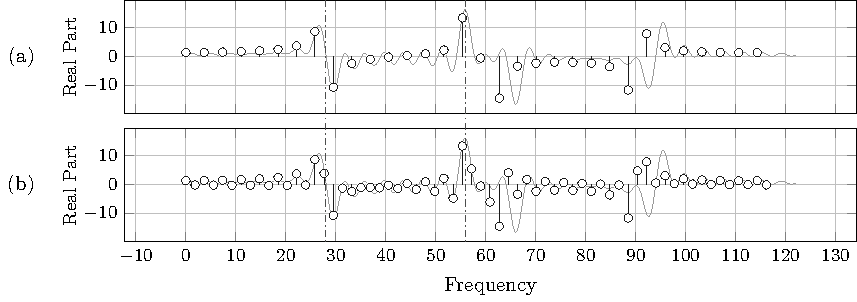
\includegraphics[height = 0.8\textheight] {tikzpics/plotCompDft32Dft64.pdf}
                    }
                    \captionof{figure} {
                        Comparing $32$ point \textsc{dft} and $64$ point \textsc{dft} of \textsc{Complex B},
                        both having \emph{sampling frequency} of \sampFreqNormJust. Also the $64$ point
                        \textsc{dtft} with the same \emph{sampling frequency} is given as a reference.
                        (a): $32$ point \textsc{dft} of \textsc{Complex B}.
                        (b): $64$ point \textsc{dft} of \textsc{Complex B}.
                    }
                    \label{fig:compDft32Dft64}
            \end{minipage}

        \end{itemize}

    \item \textbf{Mirroring of Frequencies:} Figure
        \ref{fig:wrapFreqUnitCircle} depicts an interesting physical property
        of \textsc{dtft}s. \textsc{dtft}s and \textsc{dft}s map the
        \emph{frequencies} in the $\mathcal{Z}\textsc{-plane}$ around the
        \textsc{Unit Circle}, essentially causing them to \emph{repeat} after a
        \emph{period}. From all the \textsc{dtft}s and \textsc{dft}s that we
        have taken, it is evident that the values got from \emph{sweeping} from
        $\pi$ to $2 \pi$ range\footnote{in the case of $\omega$.} is
        essentially a \emph{mirror} of values obtained\footnote{not
        \emph{always}, but the \emph{information content} will be the same.}
        from \emph{sweeping} $\omega$ from $0$ to $\pi$ range.

        \def\firstRange{$0 \si{Hz}$ to $\pgfmathprintnumber[precision = 0]{\midFreq}\si{Hz}$ }
        \def\secondRange{%
            $\pgfmathprintnumber[precision = 0]{\midFreq} \si{Hz}$ to %
            $\pgfmathprintnumber[precision = 0]{\endFreq} \si{Hz}$ %
        }

        \begin{itemize} [label=]

            \item \textbf{Sequence:} $\sin(2 \pi \freqXOne t) + j \sin(2 \pi \freqXTwo t)$

            \item
                \begin{minipage}[b] {0.85\textwidth}
                    \vspace{6pt}
                    \centering
                    \adjustbox{max width = 1\textwidth} {
                        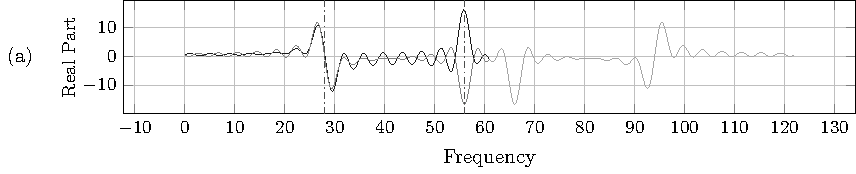
\includegraphics[height = 0.8\textheight] {tikzpics/plotFreqMirror.pdf}
                    }

                    \captionof{figure} {
                        %% TODO: range
                        Frequencies from \secondRange mirroring frequencies from \firstRange in
                        \textsc{dtft} of \textsc{Complex B}, having \emph{sampling frequency} of
                        \sampFreqSligGreatJust.
                    }
                    \label{plt:freqMirror}

                \end{minipage}

            \item
                In Figure \ref{plt:freqMirror} we can see that they don't \emph{exactly}
                overlap. This is because in our case the \emph{input sequence} was not a
                \emph{real sequence} instead it was a \emph{complex sequence}. If the
                \emph{input} was a \emph{real sequence}, the \textsc{dtft} would have
                shown so called a \emph{hermitian symmetry}\footnote{symmetry that seen
                in \emph{hermitian functions} (see the
                \textbf{\href{https://en.m.wikipedia.org/wiki/Hermitian_function}
                {Wikipedia article}}).}. Neither less, they convey the same \emph{information}. Or so
                to say, the \emph{information content} in range \firstRange \emph{mirrors
                into} \secondRange range.

        \end{itemize}

    \item \textbf{Half of Sampling Frequency:} The importance of above
        \emph{observation}\footnote{mirroring of frequencies.} is that we can
        only \emph{retrieve} or \emph{extract} the \emph{frequencies} upto
        $\frac{f_{s}}{2}$ in the case of a signal \emph{sampled} with a
        \emph{sampling frequency} of $f_{s}$. The rest will be the \emph{mirror}
        of \emph{frequencies} ranging from $0$ to $\frac{f_{s}}{2}$. In the
        case \textsc{Complex B} with \emph{sampling frequency} $122 \si{Hz}$,
        we can only \emph{extract} \emph{frequencies} upto $61 \si{Hz}$.

        \begin{itemize} [label=]

            \item \textbf{Sequence:} $\sin(2 \pi \freqXOne t) + j \sin(2 \pi \freqXTwo t)$

            \item
                \begin{minipage}[b] {0.85\textwidth}
                    \vspace{6pt}
                    \centering
                    \adjustbox{max width = 1\textwidth} {
                        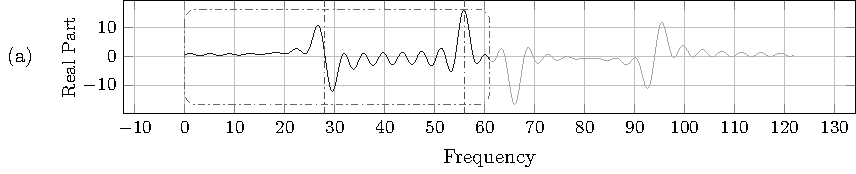
\includegraphics[height = 0.8\textheight] {tikzpics/plotHalfSampFreq.pdf}
                    }

                    \captionof{figure} {
                        Usable \emph{information} from \firstRange range in $32$ point \textsc{dtft} of
                        \textsc{Complex B} having \emph{sampling frequency} of \sampFreqSligGreatJust.
                    }
                    \label{plt:halfSampFreq}

                \end{minipage}

        \end{itemize}

    \item \textbf{Information Content:} All the plots of \textsc{dtft}s and \textsc{dft}s
        that we've plotted are actually only the \emph{real part} of the corresponding
        \emph{frequency spectrum}. But what about the \emph{imaginary part}? Let's plot
        the \emph{real part} and corresponding \emph{imaginary part} of one of the
        \emph{frequency spectrum}. Let's take \textsc{Complex B.}

        \begin{itemize} [label=]

            \item \textbf{Sequence:} $\sin(2 \pi \freqXOne t) + j \sin(2 \pi \freqXTwo t)$

            \item
                \begin{minipage}[b] {0.85\textwidth}
                    \vspace{6pt}
                    \centering
                    \adjustbox{max width = 1\textwidth} {
                        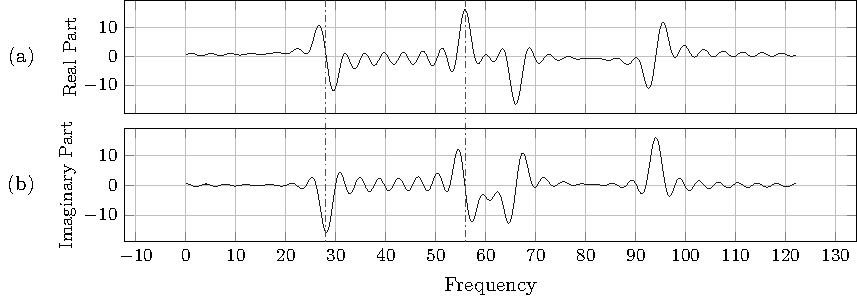
\includegraphics[height = 0.8\textheight] {tikzpics/plotCompRealImagComp.pdf}
                    }
                    \captionof{figure} {
                        Comparing \emph{real} and \emph{imaginary} parts of $32$ point \textsc{dtft}
                        of \textsc{Complex B} having \emph{sampling frequency} of \sampFreqSligGreatJust.
                        (a): \emph{Real part} of \textsc{dtft}.
                        (b): \emph{Imaginary part} of \textsc{dtft}.
                    }
                    \label{fig:compRealImagComp}
                \end{minipage}

            \item From Figure \ref{fig:compRealImagComp} we can see that we actually get
                some sense about each of the \emph{frequency components} from
                both the \emph{real} and \emph{imaginary} parts equally, but if
                we want to know where each \emph{frequency}
                belong\footnote{\label{fnt:whereBelong}like, to the \emph{real part} or the
                \emph{imaginary part}.} or the \emph{phase} of these
                \emph{frequency components}, we need to analyse both of them.
                If we are only \emph{interested} in the \emph{frequency
                components}, we could just take the \emph{absolute value} of
                our \emph{frequency spectrum}. That would give us the
                \emph{amplitude spectrum} of the \emph{frequency spectrum}.
                \emph{Amplitude spectrum} will have \emph{clean pulses}\footnote{the
                \emph{width} and the \emph{height} of these pulses will vary depending on the
                \emph{sample count}, ie, if we take \emph{higher} point \textsc{dft}, the
                \emph{pulses} will be sharp.} corresponding to each of the \emph{frequency
                components}.

        \end{itemize}

    \item \textbf{Real Part Information:} If we see any of the
        features\footnote{\label{fnt:infoMarkCircle}as inside the
        \emph{marking circles}.} like in Figure \ref{plt:realPartInfo}, in
        the \emph{real part} of the \emph{frequency spectrum}, we can conclude
        the \emph{existence} of that \emph{spectral components} in the
        \emph{input sequence}. But where\footnote{see footnote
        \ref{fnt:whereBelong}.} or what\footnote{\label{fnt:whatTheyAare}like,
        \emph{sine} or \emph{cosine} component.} they are can't be determined
        just alone from the \emph{real part}.

        \begin{itemize} [label=]

            \item \textbf{Sequence:} $\sin(2 \pi \freqXOne t) + j \sin(2 \pi \freqXTwo t)$

            \item
                \begin{minipage}[b] {0.85\textwidth}
                    \vspace{6pt}
                    \centering
                    \adjustbox{max width = 1\textwidth} {
                        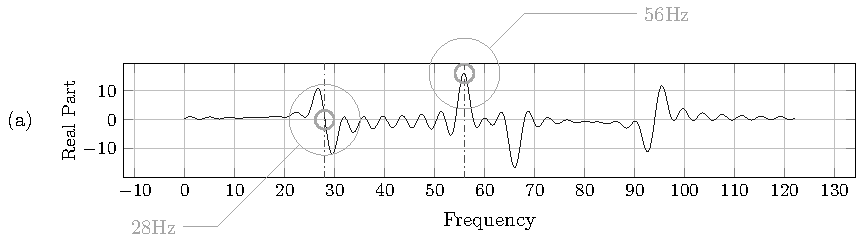
\includegraphics[height = 0.8\textheight] {tikzpics/plotRealPartInfo.pdf}
                    }
                    \captionof{figure} {
                        Features in the \emph{real part} of $32$ point \textsc{dtft} that corresponds
                        to the two \emph{frequencies} in \textsc{Complex B} having \emph{sampling frequency}
                        of \sampFreqSligGreatJust.
                    }
                    \label{plt:realPartInfo}
                \end{minipage}

        \end{itemize}

    \item \textbf{Imaginary Part Information:} If we see any of the features\footnote{see
        footnote \ref{fnt:infoMarkCircle}} like in Figure \ref{plt:imagPartInfo}, in
        the \emph{imaginary part} of the \emph{frequency spectrum}, we can conclude
        the \emph{existence} of that \emph{spectral components} in the
        \emph{input sequence}. But where\footnote{see footnote \ref{fnt:whereBelong}.}
        or what\footnote{see footnote \ref{fnt:whatTheyAare}.} they are can't be determined
        just alone from the \emph{imaginary part}.

        \begin{itemize} [label=]

            \item \textbf{Sequence:} $\sin(2 \pi \freqXOne t) + j \sin(2 \pi \freqXTwo t)$

            \item
                \begin{minipage}[b] {0.85\textwidth}
                    \vspace{6pt}
                    \centering
                    \adjustbox{max width = 1\textwidth} {
                        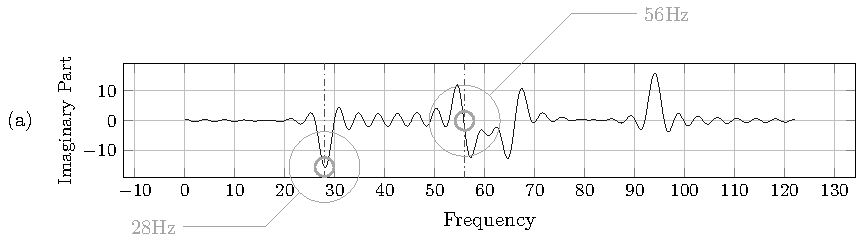
\includegraphics[height = 0.8\textheight] {tikzpics/plotImagPartInfo.pdf}
                    }
                    \captionof{figure} {
                        Features in the \emph{imaginary part} of $32$ point \textsc{dtft} that corresponds
                        to the two \emph{frequencies} in \textsc{Complex B} having \emph{sampling frequency}
                        of \sampFreqSligGreatJust.
                    }
                    \label{plt:imagPartInfo}
                \end{minipage}

        \end{itemize}

    \item \textbf{Way Higher Sampling Frequency:} In Figure \ref{plt:higherSampFreq} we can almost
        see the two \emph{frequencies}. But if we \emph{increase} the \emph{sampling frequency} again
        without \emph{increasing} the \emph{sample count}\footnote{in our case it was $32$ and $64$.},
        the \textsc{dtft} or \textsc{dft} might lose those \emph{frequency information}.
        It seems like we need to \emph{increase} the \emph{sample count} as well as the
        \emph{sampling frequency} in order to get a proper \emph{frequency spectrum}.

        \pagebreak

        \begin{itemize} [label=]

            \item \textbf{Sequence:} $\sin(2 \pi \freqXOne t) + j \sin(2 \pi \freqXTwo t)$

            \item
                \begin{minipage}[b] {0.85\textwidth}
                    \vspace{6pt}
                    \centering
                    \adjustbox{max width = 1\textwidth} {
                        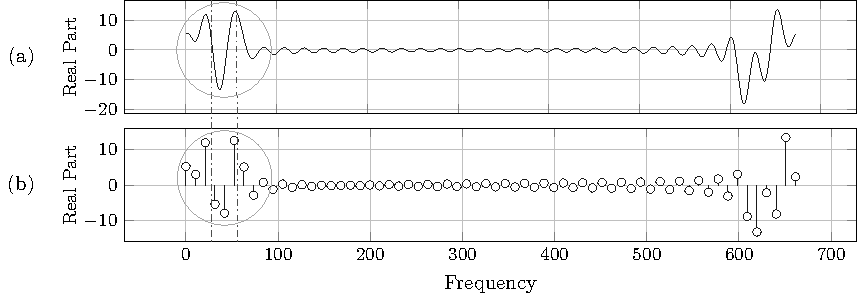
\includegraphics[height = 0.8\textheight] {tikzpics/plotHigherSampFreq.pdf}
                    }
                    \captionof{figure} {
                        $64$ point \textsc{dtft} and \textsc{dft} of \textsc{Complex B}, both
                        having \emph{sampling frequency} of \sampFreqSligGreatJust.
                        (a): $64$ point \textsc{dtft}.
                        (b): $64$ point \textsc{dft}.
                    }
                    \label{plt:higherSampFreq}
                \end{minipage}

        \end{itemize}

    \item \textbf{Detection of Closer Frequencies:} From the \textsc{dtft}s and \textsc{dft}s
        of \textsc{Complex F} from Section \ref{ssec:visCplxF}, we can see that it is hard to
        distinguish between the \emph{closer frequencies} like $\freqXTwo \si{Hz}$ and
        $\freqXThree \si{Hz}$.

        \begin{itemize} [label=]

            \item \textbf{Sequence:} $\sin(2 \pi \freqXTwo t) + j \sin(2 \pi \freqXThree t)$

            \item
                \begin{minipage}[b] {0.85\textwidth}
                    \vspace{6pt}
                    \centering
                    \adjustbox{max width = 1\textwidth} {
                        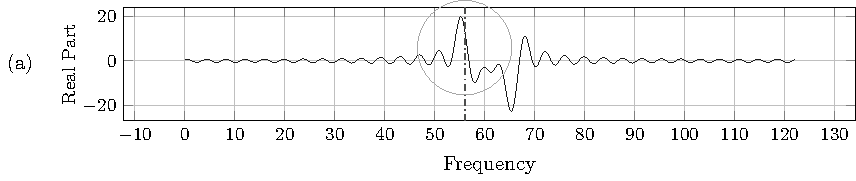
\includegraphics[height = 0.8\textheight] {tikzpics/plotDtftCloseFreq.pdf}
                    }
                    \captionof{figure} {
                        $\freqXTwo \si{Hz}$ and $\freqXThree \si{Hz}$ being \emph{undistinguishable} from $32$
                        point \textsc{dtft} of \textsc{Complex F} having \emph{sampling frequency} of
                        \sampFreqSligGreatJust.
                    }
                    \label{plt:dtftCloseFreq}
                \end{minipage}

            \item
                \begin{minipage}[b] {0.85\textwidth}
                    \vspace{6pt}
                    \centering
                    \adjustbox{max width = 1\textwidth} {
                        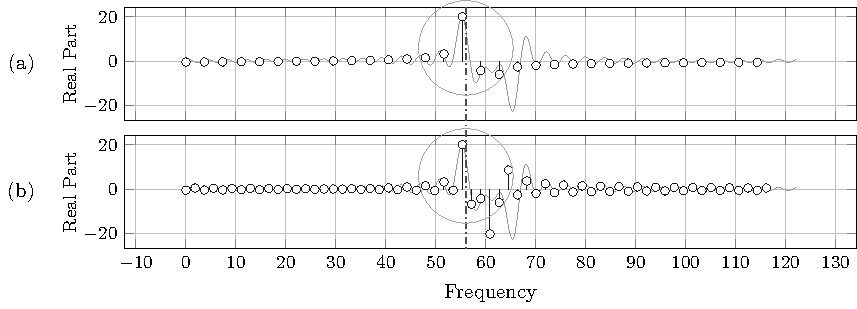
\includegraphics[height = 0.8\textheight] {tikzpics/plotDftCloseFreq.pdf}
                    }
                    \captionof{figure} {
                        $32$ point \textsc{dft} and $64$ point \textsc{dft} with corresponding \textsc{N} point
                        \textsc{dtft}s of \textsc{Complex F} with \emph{sampling frequency} of \sampFreqSligGreatJust,
                        still having \emph{undistinguishable} \emph{frequency components}.
                        (a): $32$ point \textsc{dft} with $32$ point \textsc{dtft}.
                        (b): $64$ point \textsc{dft} with $64$ point \textsc{dtft}.
                    }
                    \label{plt:dftCloseFreq}
                \end{minipage}

            \item
                As we can see from Figure \ref{plt:dtftCloseFreq} and \ref{plt:dftCloseFreq}, the
                \emph{close frequencies} $\freqXTwo \si{Hz}$ and $\freqXThree \si{Hz}$ are
                \emph{undistinguishable} from each other. As we can see from Figure \ref{plt:dftCloseFreq}
                the \emph{zero padding} doesn't seem to help much in this regard. Even if we
                \emph{zero pad} to a \emph{higher length} and took the \textsc{dft}, we will only
                going to get something similar to the \textsc{dtft} in Figure \ref{plt:dtftCloseFreq}.
                But there is another way to be able to \emph{distinguish} between \emph{closer
                frequencies}, that is to take a \emph{higher number} of \emph{samples}\footnote{not
                as same as \emph{zero padding}.} and then take a \emph{higher point} \textsc{dft}.
                Instead of taking $32$ or $64$ \emph{samples}, if we take a \emph{higher sample
                count}\footnote{let's say $1024$ samples.} and then take a \emph{higher point}
                \textsc{dft} we might be able to get that high of a \emph{frequency resolution}.

        \end{itemize}

\end{itemize}

\end{document}
